\section{Concatenation}

\frame{\tableofcontents[currentsection]}

\begin{frame}
    \frametitle{Problem Statement}
    \begin{center} \ttfamily
         [1,2,3,4,5] ++ [6,7,8,9,10,11,12,13]\\[4mm]
         $\downarrow$ \\[4mm]
         [1,2,3,4,5,6,7,8,9,10,11,12,13]
    \end{center}
\end{frame}

\begin{frame}
    \frametitle{Updating an Array}
    \begin{center}
        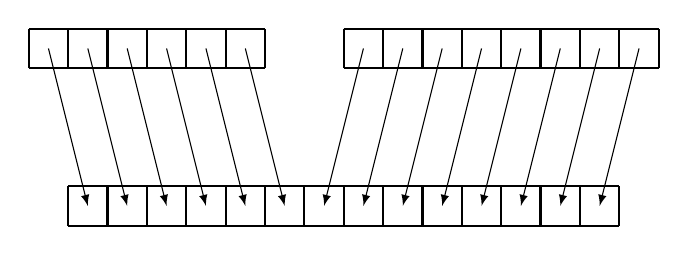
\begin{tikzpicture}
            \draw[thick] (0,0) grid[step=0.5cm] ++(3,0.5);
            \draw[thick,xshift=4cm] (0,0) grid[step=0.5cm] ++(4,0.5);
            \draw[thick,xshift=0.5cm] (0,-2) grid[step=0.5cm] ++(7,0.5);

            \foreach \i in {0,0.5,...,2.5} {
                \draw[-latex] (\i+0.25,0.25) -- (\i+0.75,-1.75);
            }

            \foreach \i in {0,0.5,...,3.5} {
                \draw[-latex] (\i+4.25,0.25) -- (\i+3.75,-1.75);
            }
        \end{tikzpicture}
    \end{center}
    \vskip4mm
    \structure{Algorithm}
    \begin{itemize}
        \item Requires both arries to be copied
        \item $O(n_1 + n_2)$
    \end{itemize}
\end{frame}

\begin{frame}
    \frametitle{Updating a Linked List}
    \begin{center}
        \begin{tikzpicture}[link/.style={thick,-latex}]
            \foreach[count=\i] \x in {0,...,4} {
                \coordinate (p\i) at (\x,0);
                \llnode[position=p\i,size=0.25cm]
            }

            \foreach[evaluate={\i+1} as \j] \i in {1,...,4} {
                \draw[-latex] ($ (p\i) + (0.375,0.125) $) -- ($ (p\j) + (0,0.125) $);
            }

            \foreach[count=\i] \x in {0,...,8} {
                \coordinate (q\i) at (\x,-0.5);
                \llnode[position=q\i,size=0.25cm]
            }

            \foreach[evaluate={\i+1} as \j] \i in {1,...,8} {
                \draw[-latex] ($ (q\i) + (0.375,0.125) $) -- ($ (q\j) + (0,0.125) $);
            }

            \foreach[count=\i] \x in {0,...,4} {
                \coordinate (r\i) at (\x,-2);
                \llnode[position=r\i,size=0.25cm]
            }

            \foreach[evaluate={\i+1} as \j] \i in {1,...,4} {
                \draw[-latex] ($ (r\i) + (0.375,0.125) $) -- ($ (r\j) + (0,0.125) $);
            }
            \draw[-latex] ($ (r5) + (0.375,0.125) $) -- ($ (q1) + (0.25,0) $);
        \end{tikzpicture}
    \end{center}
    \vskip4mm
    \structure{Algorithm}
    \begin{itemize}
        \item Only first list needs to be copied
        \item Second list can be safely reused
        \item Copy's last node points to second list's first node
        \item $O(n_1)$
    \end{itemize}
\end{frame}
